\section{Reward score distributions for FP8 mitigations}
\label{section:fp8appendix}

Figure \ref{figure:reward-skip} shows how much the reward score distribution changes if we do not skip the first and last layers during FP8 quantization. It is possible to note a significant shift in the distribution, showing the importance of this change to the model quality.

\begin{figure}[t]
\centering
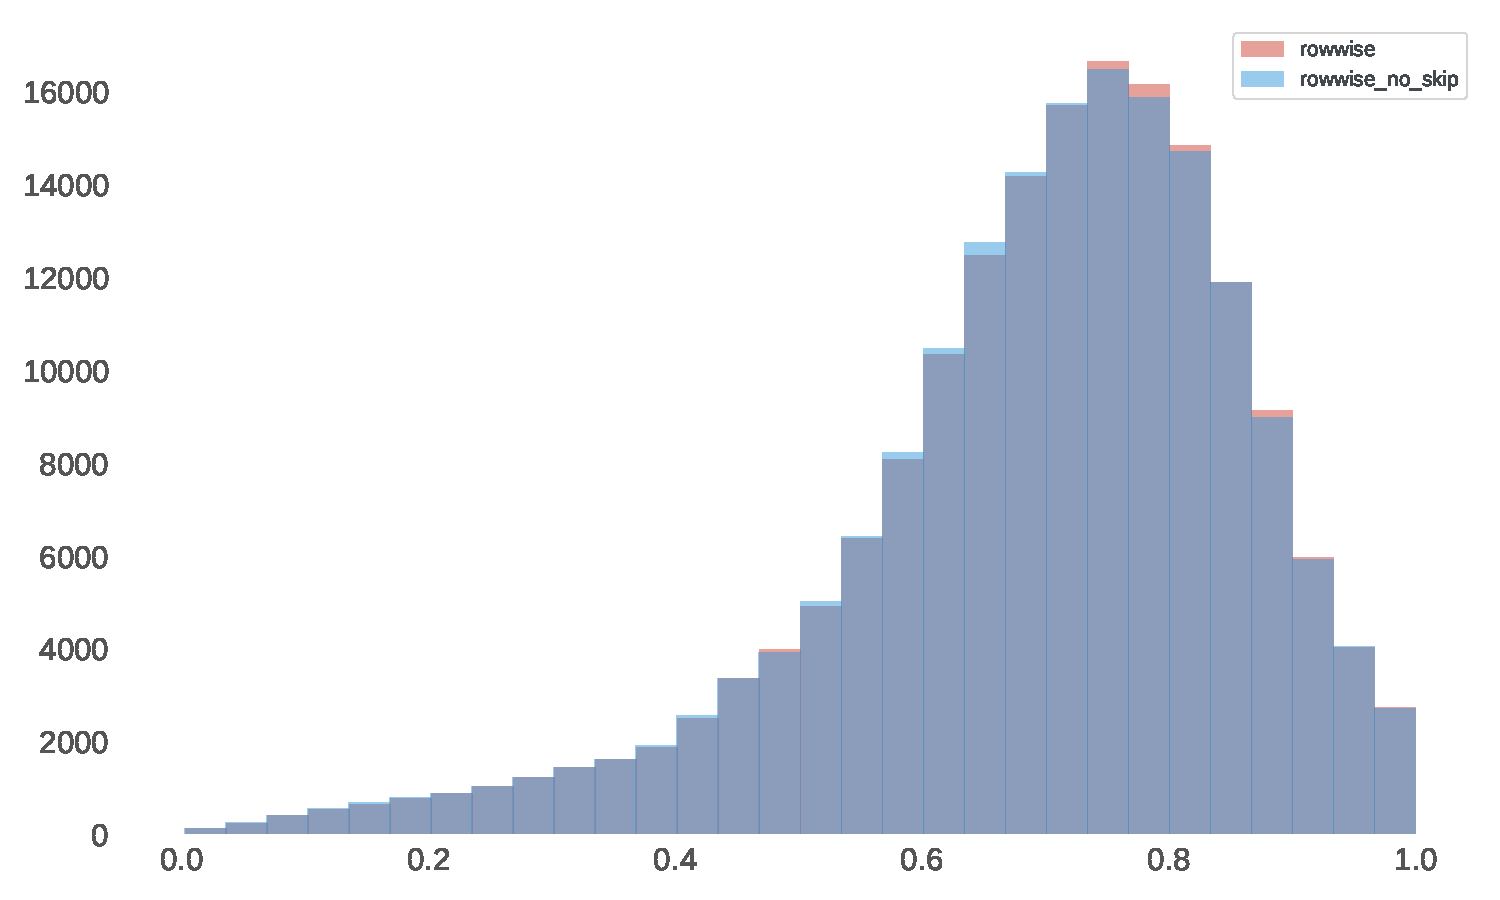
\includegraphics[scale=0.5]{assets/fp8_row_vs_fp8_row_no_skip_data.pdf}
\caption{Reward score distribution for 405B using FP8 with and without skipping the first and last transformer layers}
\label{figure:reward-skip}
\end{figure}

Figure \ref{figure:reward-ub} shows that the addition of the static upper-bound for the dynamic activation scales doesn't have as big of an impact on the row-wise kernel in terms of quality, when compared to skipping layers. However, the change is still noticeable and we include it as an extra layer of protection to prevent against some rare corruptions.

\begin{figure}[t]
\centering
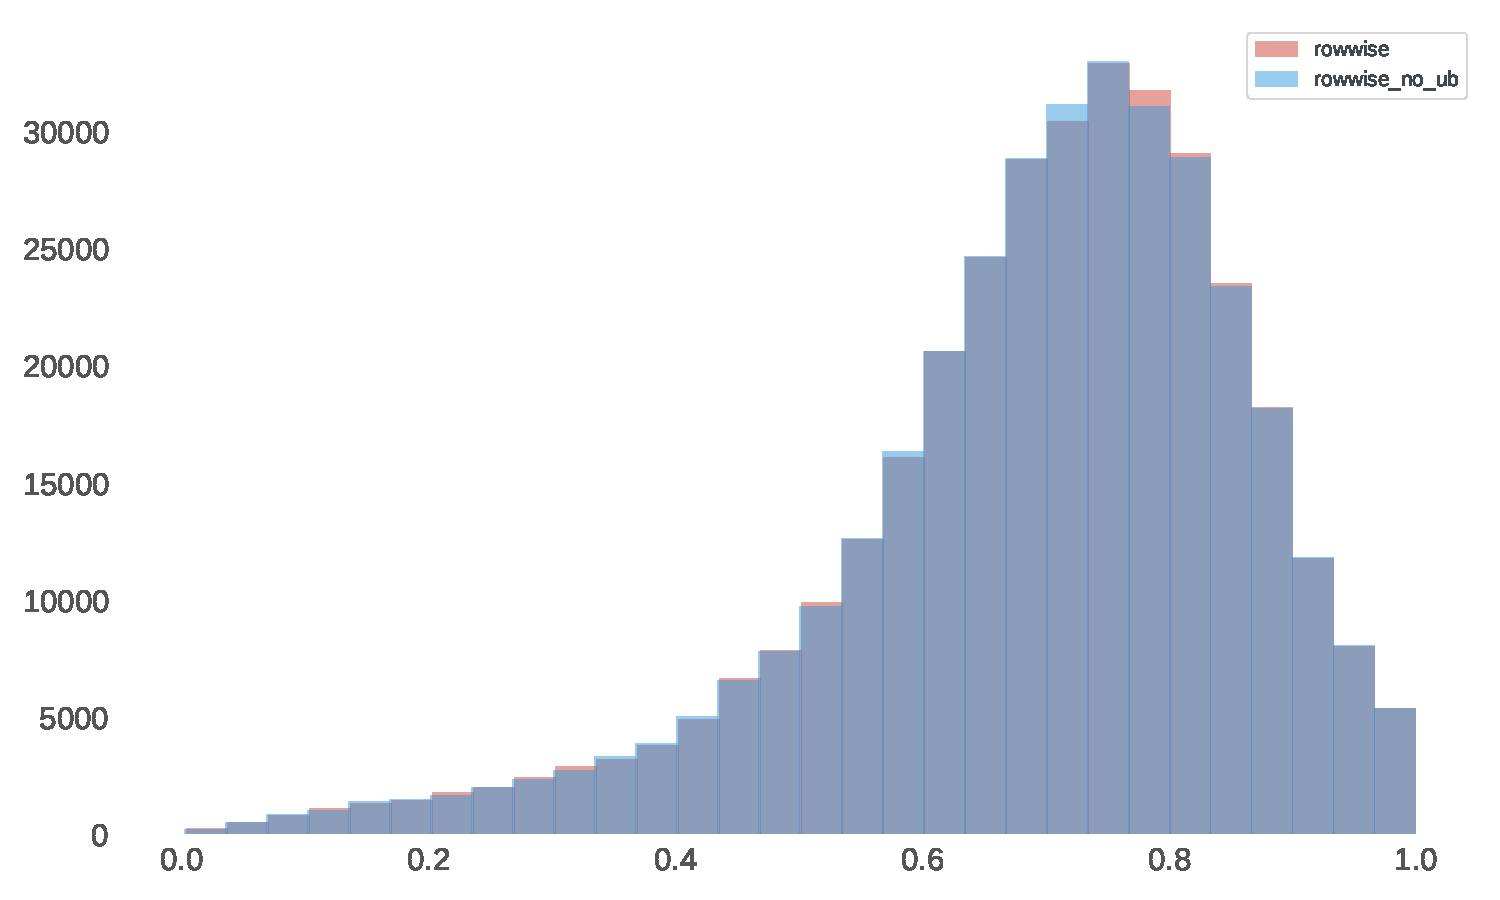
\includegraphics[scale=0.5]{assets/fp8_row_vs_fp8_row_no_ub_data.pdf}
\caption{Reward score distribution for 405B using FP8 with and without including the static upper-bound for activation scales}
\label{figure:reward-ub}
\end{figure}

Figure \ref{figure:reward-tensor} shows that the tensor-wise kernel is slightly less accurate than row-wise.

\begin{figure}[t]
\centering
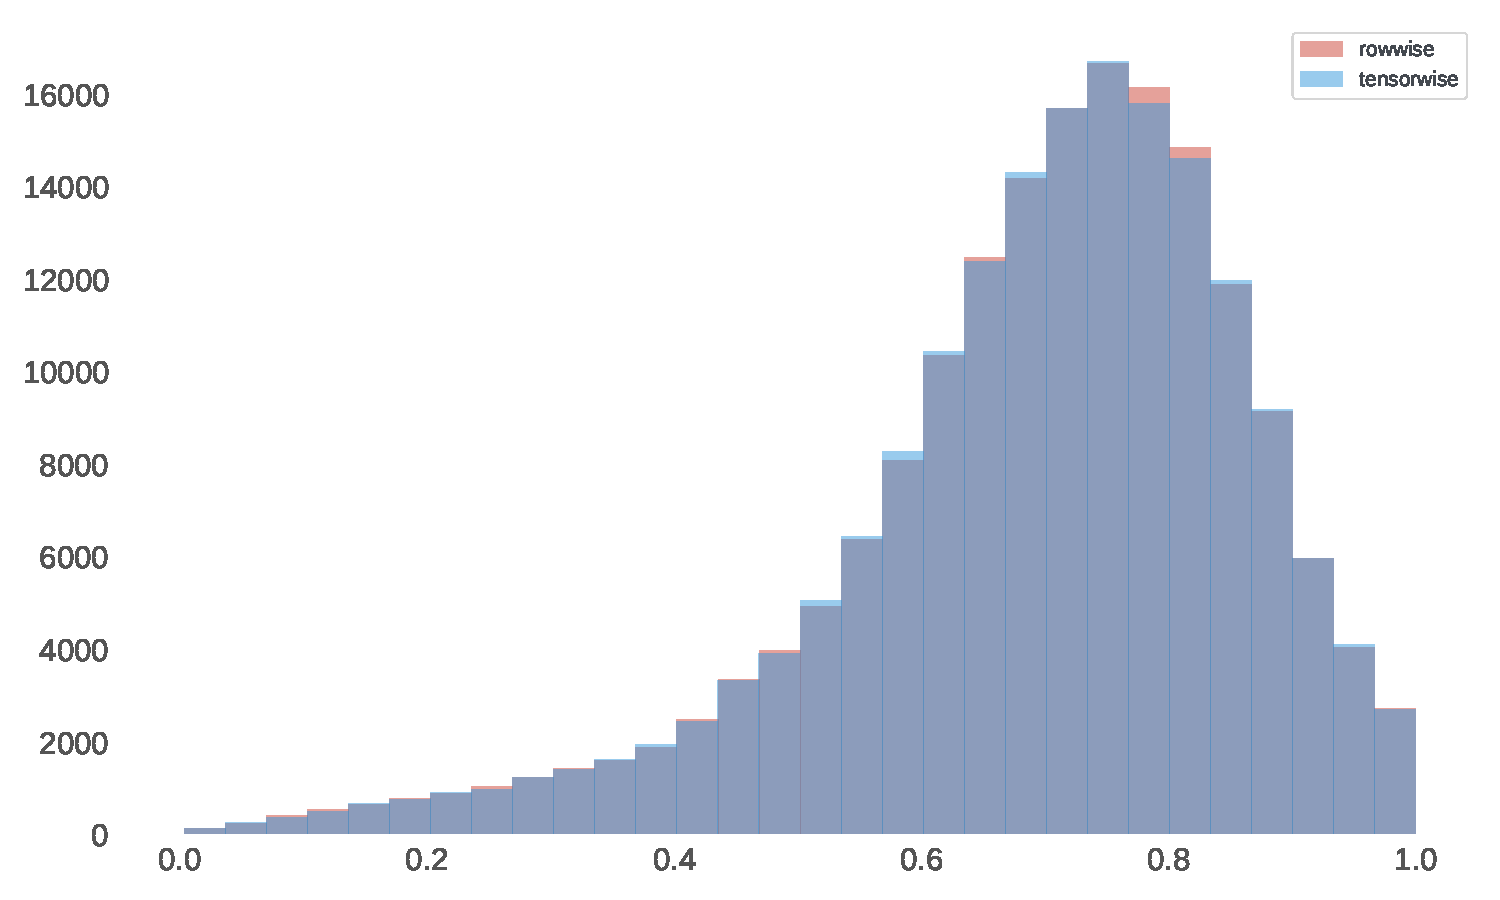
\includegraphics[scale=0.5]{assets/row_vs_tensor.pdf}
\caption{Reward score distribution for 405B using FP8 with the tensor-wise and row-wise kernels}
\label{figure:reward-tensor}
\end{figure}
